\documentclass{beamer}
\usepackage{graphicx}
\usepackage[utf8]{inputenc}

\usetheme{Antibes}
\author{Nicolas ENNAJI, Sylvain MARCHAND}
\title{Déploiement des agents composant une Smart Grid dans des micro-contrôleurs}

\begin{document}

\begin{frame}
\titlepage

\end{frame}

%%%%%%%%%%%%%%%%%%%%%%%%%%%%%%%%%%%%%%%%%%%%%%%%%%%%%%%%%%%%%%%%%%%%%%%%%%%%%%%

\begin{frame}
\frametitle{Plan}
\tableofcontents

\end{frame}

%%%%%%%%%%%%%%%%%%%%%%%%%%%%%%%%%%%%%%%%%%%%%%%%%%%%%%%%%%%%%%%%%%%%%%%%%%%%%%%
\section{Le principe}

\begin{frame}
\frametitle{Le principe}

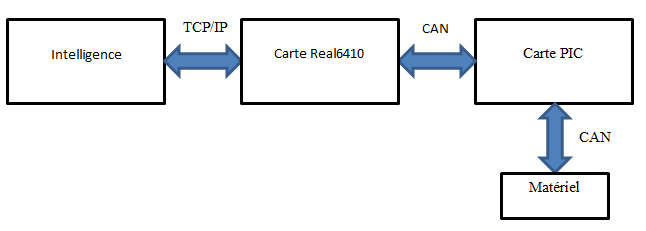
\includegraphics[width=1\textwidth]{images/Recap.png}


\end{frame}

%%%%%%%%%%%%%%%%%%%%%%%%%%%%%%%%%%%%%%%%%%%%%%%%%%%%%%%%%%%%%%%%%%%%%%%%%%%%%%%
\section{Le matériel}

\begin{frame}
\frametitle{Le matériel}
\begin{itemize}
\item Real6410 \\
  $\rightarrow$ mcp2515 : transforme du spi en CAN
\item Carte dsPIC33F \\
  $\rightarrow$ mcp2551 : transforme du spi en CAN
\end{itemize}

\end{frame}
%%%%%%%%%%%%%%%%%%%%%%%%%%%%%%%%%%%%%%%%%%%%%%%%%%%%%%%%%%%%%%%%%%%%%%%%%%%%%

\section{La communication}

\begin{frame}
\frametitle{La communication IA - cartes}
\begin{itemize}
  \item Socket tcp
  \item Mise en forme des données pour le PIC
\end{itemize}

\end{frame}
%%%%%%%%%%%%%%%%%%%%%%%%%%%%%%%%%%%%%%%%%%%%%%%%%%%%%%%%%%%%%%%%%%%%%%%%%%%%%
\begin{frame}
\frametitle{La communication Real6410 - carte PIC}
\begin{itemize}
  \item Utilisation du bus CAN
  \item Résistant aux interférences
  \item Portée assez longue
\end{itemize}

\end{frame}
%%%%%%%%%%%%%%%%%%%%%%%%%%%%%%%%%%%%%%%%%%%%%%%%%%%%%%%%%%%%%%%%%%%%%%%%%%%%%
\section{L'implémentation}

\begin{frame}
\frametitle{Côté Real6410}
\begin{itemize}
  \item Driver inclus dans le noyau Linux $\rightarrow$ écriture sur le driver impossible
  \item Interface réseau non présente $\rightarrow$ recompilation du noyau.
  \item Problème d'interface : le programme iproute non fonctionnel
  \item Interface 'vcan' non activée
  \item Interface CAN RAW non activée
\end{itemize}
\end{frame}
%%%%%%%%%%%%%%%%%%%%%%%%%%%%%%%%%%%%%%%%%%%%%%%%%%%%%%%%%%%%%%%%%%%%%%%%%%%%%
\begin{frame}
\frametitle{Côté PIC}
\begin{itemize}
  \item Module eCAN.
  \item Utilisation de la DMA.
  \item Initialisation avec identifiants standard.
  \item Envoie/réception de messages.
  \item Testé en mode loopback.
\end{itemize}

\end{frame}
%%%%%%%%%%%%%%%%%%%%%%%%%%%%%%%%%%%%%%%%%%%%%%%%%%%%%%%%%%%%%%%%%%%%%%%%%%%%%
\section{Résultats}
\begin{frame}
\frametitle{Résultats}
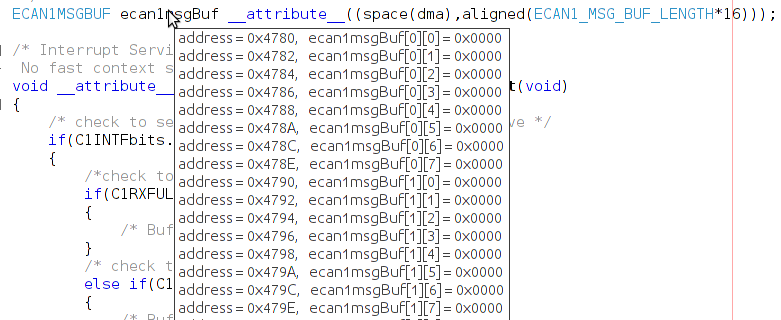
\includegraphics[width=0.8\textwidth]{images/CAN_avant_envoi.png}
\end{frame}
%%%%%%%%%%%%%%%%%%%%%%%%%%%%%%%%%%%%%%%%%%%%%%%%%%%%%%%%%%%%%%%%%%%%%%%%%%%%%
\section{Résultats}
\begin{frame}
\frametitle{Résultats}
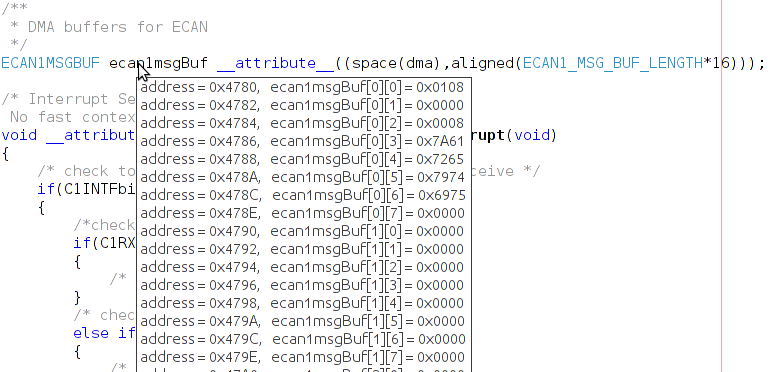
\includegraphics[width=0.8\textwidth]{images/CAN_avant_reception.png}
\end{frame}
%%%%%%%%%%%%%%%%%%%%%%%%%%%%%%%%%%%%%%%%%%%%%%%%%%%%%%%%%%%%%%%%%%%%%%%%%%%%%
\section{Résultats}
\begin{frame}
\frametitle{Résultats}
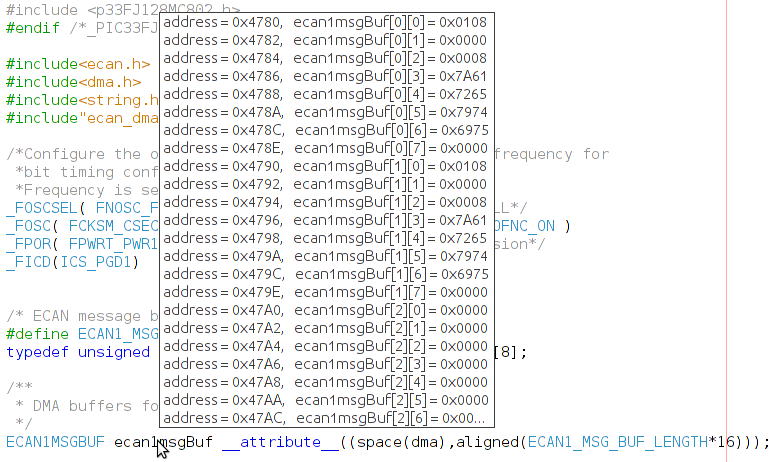
\includegraphics[width=0.8\textwidth]{images/CAN_apres_reception.png}
\end{frame}
%%%%%%%%%%%%%%%%%%%%%%%%%%%%%%%%%%%%%%%%%%%%%%%%%%%%%%%%%%%%%%%%%%%%%%%%%%%%%
\section{Bilan}
\begin{frame}
\frametitle{Bilan}
\begin{itemize}
  \item Carte Real6410 non fonctionnelle en CAN
  \item Carte PIC fonctionnelle en CAN
  \item Carte Real6410 : une TX pour EE ?
\end{itemize}
\end{frame}
%%%%%%%%%%%%%%%%%%%%%%%%%%%%%%%%%%%%%%%%%%%%%%%%%%%%%%%%%%%%%%%%%%%%%%%%%%%%%
\begin{frame}
\begin{center}
Merci pour votre attention.
\end{center}
\end{frame}


\end{document}
